\section{可测映射}
\label{sec:meas-measurable-maps}

有了测度，下一步是把它用到函数上：一根细杆各处的线密度不同，总质量是多少；一个随机实验的结果被读成一个数，这个数落在某个区间里的概率是多少。每当对函数的输出提出“是否落在某集合中”的问题，就需要在输入端测量相应的点集。本节用原像刻画这一要求，先给出可测映射的定义与判据，再证明数值函数的常见运算和可数极限保持可测性，最后用只取有限个值的简单函数从下方逼近非负可测函数，为下一章定义积分准备对象。

\subsection{可测映射}
\label{sec:meas-measurable-map-def}

\paragraph{原像与可测性}
对映射$f:X\to Y$与$B\subseteq Y$，原像$f^{-1}(B)=\{x\in X:f(x)\in B\}$是“输出落在$B$中”的那些输入。原像对任意映射都有意义，并不要求$f$可逆。若输出端能提出的每个集合问题，在输入端都对应一个可测集合，就说$f$可测。

\begin{definition}[可测映射]
\label{def:meas-measurable-map}
设$(X,\mathcal A)$、$(Y,\mathcal B)$是可测空间。若对每个$B\in\mathcal B$都有$f^{-1}(B)\in\mathcal A$，称映射$f:X\to Y$为$\mathcal A/\mathcal B$-\term{可测映射}（measurable map），简称可测。
\end{definition}

可测性同时取决于两端的$\sigma$代数。在$X=\{1,2,3,4\}$上取由$\varnothing,\{1,2\},\{3,4\},X$组成的$\sigma$代数$\mathcal A$，在$Y=\{a,b\}$上取$\mathcal P(Y)$。令$f(1)=f(2)=a$、$f(3)=f(4)=b$，则$f^{-1}(\{a\})=\{1,2\}$、$f^{-1}(\{b\})=\{3,4\}$都可测，$f$可测。令$g(1)=a$、$g(2)=g(3)=g(4)=b$，则$g^{-1}(\{a\})=\{1\}\notin\mathcal A$，$g$不可测：输入端只知道点属于哪一组，无法回答“输出是否为$a$”。若把$Y$上的$\sigma$代数换成$\{\varnothing,Y\}$，$g$又变成可测的，因为输出端不再提出任何非平凡问题。

这与连续性的定义形式相同，内容不同。第~\ref{chap:topological-spaces}章的连续映射要求开集的原像是开集，可测映射要求可测集的原像是可测集。连续性关心邻近关系是否保持，可测性只关心集合问题能否在输入端回答，与距离和开集没有直接关系。

\paragraph{生成族判据}
直接检查$\mathcal B$中的每个集合往往做不到，例如$\mathcal B(\mathbb R)$中的集合无法逐一列出。原像与集合运算可交换，所以只需检查生成族。

\begin{lemma}[生成族判据]
\label{lem:meas-generator-criterion}
设$\mathcal B=\sigma(\mathcal C)$。若对每个$C\in\mathcal C$都有$f^{-1}(C)\in\mathcal A$，则$f$是$\mathcal A/\mathcal B$可测的。
\end{lemma}

\begin{proof}
令$\mathcal E=\{B\subseteq Y:f^{-1}(B)\in\mathcal A\}$。由$f^{-1}(Y)=X$、$f^{-1}(Y\setminus B)=X\setminus f^{-1}(B)$与$f^{-1}(\bigcup_nB_n)=\bigcup_nf^{-1}(B_n)$，$\mathcal E$是$Y$上的$\sigma$代数。它含$\mathcal C$，所以含$\sigma(\mathcal C)=\mathcal B$。
\end{proof}

由定义还可以直接得到复合规则。若$f:(X,\mathcal A)\to(Y,\mathcal B)$与$g:(Y,\mathcal B)\to(Z,\mathcal C)$都可测，则对$C\in\mathcal C$，$(g\circ f)^{-1}(C)=f^{-1}(g^{-1}(C))\in\mathcal A$，所以$g\circ f$可测。这里要求中间空间$Y$上两次使用的是同一个$\sigma$代数$\mathcal B$。

\paragraph{可测函数}
最常用的可测映射取实数值。目标端取$\mathcal B(\mathbb R)$；允许取$\pm\infty$时，在扩展实数$[-\infty,+\infty]$上取由$\mathcal B(\mathbb R)$与两个单点$\{-\infty\},\{+\infty\}$生成的$\sigma$代数。由定理~\ref{thm:meas-borel-generators}，半直线$(a,+\infty)$生成$\mathcal B(\mathbb R)$，再加上$\{+\infty\}=\bigcap_n(n,+\infty]$与$\{-\infty\}=[-\infty,+\infty]\setminus\bigcup_n(-n,+\infty]$，可知$(a,+\infty]$生成扩展实数上的这个$\sigma$代数。判据于是化为检查阈值集合。

\begin{definition}[可测函数]
\label{def:meas-measurable-function}
设$(X,\mathcal A)$是可测空间。若$f:X\to[-\infty,+\infty]$对每个$a\in\mathbb R$都有$\{f>a\}=\{x:f(x)>a\}\in\mathcal A$，称$f$为\term{可测函数}（measurable function）。当$(X,\mathcal A)=(\mathbb R^d,\mathcal B(\mathbb R^d))$时，称为\term{Borel可测函数}（Borel measurable function）。
\end{definition}

由生成族判据，实值函数$f$可测等价于它是$\mathcal A/\mathcal B(\mathbb R)$可测映射；只检查有理数$a$也够用。用补集与可数运算还可得到其他阈值集合，例如$\{f\geq a\}=\bigcap_n\{f>a-1/n\}$、$\{f\leq a\}=X\setminus\{f>a\}$，它们都可测。复值函数$f=u+\mathrm iv$称为可测，是指实部$u$与虚部$v$都可测。

集合的可测性与函数的可测性通过指示函数相连。对$A\subseteq X$，$\{\mathbf 1_A>a\}$在$a<0$时为$X$，在$0\leq a<1$时为$A$，在$a\geq1$时为$\varnothing$，所以$\mathbf 1_A$可测当且仅当$A\in\mathcal A$。例如$\mathbf 1_{\mathbb Q}$在$(\mathbb R,\mathcal B(\mathbb R))$上可测，因为$\mathbb Q$是Borel集；第~\ref{sec:meas-jordan}小节中它对应的集合连Jordan可测都不是。

\paragraph{连续映射与可测性}
设$X,Y$是度量空间，$f:X\to Y$连续。开集的原像是开集，因而属于$\mathcal B(X)$；开集生成$\mathcal B(Y)$，由生成族判据，$f$是$\mathcal B(X)/\mathcal B(Y)$可测的。所以连续函数都是Borel可测函数。

逆向结论不成立。阶跃函数$H=\mathbf 1_{[0,+\infty)}$的阈值集合是$\mathbb R$、$[0,+\infty)$或$\varnothing$，都是Borel集，所以$H$是Borel可测函数，但它在$0$处不连续；$\mathbf 1_{\mathbb Q}$处处不连续，却同样Borel可测。可测性只问阈值集合是否在允许测量的集合族里，对函数的局部变化没有任何要求。

上面的结论依赖两端都取Borel结构。若把两端都换成Lebesgue可测集$\mathcal L$，连续函数$f:\mathbb R\to\mathbb R$未必$\mathcal L/\mathcal L$可测：可以构造连续严格单调的$f$与零测集的子集$S$（由完备性，$S\in\mathcal L$），使$f^{-1}(S)$不Lebesgue可测。这里不展开构造，只记住：可测性必须写清两端的集合族，不能把目标端的Borel结构随意换成某个测度的完备化。本书中实值函数的目标端总取Borel结构。

\subsection{可测函数的运算}
\label{sec:meas-function-operations}

\paragraph{代数运算}
可测函数经过加、乘、取绝对值等运算后仍然可测。困难在于和的阈值集合$\{f+g>a\}$不能直接写成$f$与$g$各自阈值集合的有限组合，需要用有理数作可数分拆。

\begin{theorem}[可测函数的运算]
\label{thm:meas-function-operations}
设$f,g:X\to\mathbb R$可测，$c\in\mathbb R$，$\varphi:\mathbb R\to\mathbb R$连续。则$cf$、$f+g$、$\varphi\circ f$、$fg$、$\lvert f\rvert$、$\max\{f,g\}$、$\min\{f,g\}$都可测；若$g$处处不为零，$f/g$也可测。
\end{theorem}

\begin{proof}
$\varphi\circ f$是可测映射与Borel可测的连续函数之复合，所以可测。取$\varphi(t)=ct$、$\lvert t\rvert$、$t^2$，得$cf$、$\lvert f\rvert$、$f^2$可测。

对和，若$f(x)+g(x)>a$，则$f(x)>a-g(x)$，在两者之间取有理数$q$，有$f(x)>q$且$g(x)>a-q$；反之这两式蕴含$f(x)+g(x)>a$。所以
\[
 \{f+g>a\}=\bigcup_{q\in\mathbb Q}\bigl(\{f>q\}\cap\{g>a-q\}\bigr),
\]
是可数个可测集合之并。于是$f-g=f+(-1)g$可测。积由$fg=\tfrac14\bigl((f+g)^2-(f-g)^2\bigr)$得到，最大值与最小值由$\max\{f,g\}=\tfrac12(f+g+\lvert f-g\rvert)$与$\min\{f,g\}=\tfrac12(f+g-\lvert f-g\rvert)$得到。若$g$处处非零，$t\mapsto1/t$在$\mathbb R\setminus\{0\}$上连续，把它在$0$处任意赋值得到的Borel函数与$g$复合，可知$1/g$可测，从而$f/g$可测。
\end{proof}

复值可测函数按实部与虚部计算，同样对加法、乘法和取模封闭：$\lvert f\rvert=\sqrt{u^2+v^2}$是连续函数作用于$(u,v)$，可以先由$u^2+v^2$可测再取平方根。

\paragraph{扩展实值的运算范围}
允许取扩展实数值时，运算本身可能没有定义。$f+g$在$f(x)=+\infty$、$g(x)=-\infty$的点没有意义，必须先说明这样的点不出现，或者在那里另作约定；乘积还要约定$0\cdot(\pm\infty)$，本书取$0\cdot(\pm\infty)=0$。只有在这些点上的值确定以后，才能谈论运算结果是否可测。非负可测函数的和总有定义，并且可测：$\{f+g>a\}$在上式之外还要并上$\{f=+\infty\}\cup\{g=+\infty\}$。

\paragraph{函数列的上下确界与极限}
分析中的许多函数作为函数列的极限得到，例如级数的和与逐次逼近的结果。下一章的收敛定理正要处理这类极限，所以先确认极限对象仍然可测。

\begin{theorem}[可数极限的可测性]
\label{thm:meas-limits}
设$f_1,f_2,\dots:X\to[-\infty,+\infty]$可测。则$\sup_nf_n$、$\inf_nf_n$、$\limsup_nf_n$、$\liminf_nf_n$可测。若对每个$x$，极限$\lim_nf_n(x)$在$[-\infty,+\infty]$中存在，则极限函数可测。
\end{theorem}

\begin{proof}
$\sup_nf_n(x)>a$当且仅当某个$f_n(x)>a$，所以$\{\sup_nf_n>a\}=\bigcup_n\{f_n>a\}$可测。由$\inf_nf_n=-\sup_n(-f_n)$得下确界可测。上极限与下极限是可数次上、下确界的组合：
\[
 \limsup_{n\to\infty}f_n=\inf_{n\geq1}\sup_{k\geq n}f_k,\qquad \liminf_{n\to\infty}f_n=\sup_{n\geq1}\inf_{k\geq n}f_k,
\]
由前两步可测。极限存在时它等于上极限，因而可测。
\end{proof}

可数性在证明中不可缺少。设$S\subseteq\mathbb R$不是Borel集，对每个$s\in S$，$\mathbf 1_{\{s\}}$都是Borel可测函数，但它们的逐点上确界$\mathbf 1_S$不是，因为$\{\mathbf 1_S>0\}=S$。指标不可数时，$\{\sup_sf_s>a\}$是不可数并，$\sigma$代数不保证它可测。这个定理也只保证极限对象可测，不说明极限函数的积分等于积分的极限，那是下一章收敛定理的内容。

\paragraph{零测修改}
函数在零测集上的取值通常无关紧要，但修改后的函数是否仍然可测，取决于测度空间是否完备。设$f$可测，$g$与$f$只在某个零测集$N$内可能不同。若空间完备，则$\{g>a\}=(\{f>a\}\setminus N)\cup(\{g>a\}\cap N)$，第一项可测，第二项是零测集的子集，所以$g$可测。

若空间不完备，结论可能失败。在第~\ref{sec:meas-completion}小节的例子中，$X=\{1,2,3\}$，$\mathcal A=\{\varnothing,\{1\},\{2,3\},X\}$，$\mu=\delta_1$。取$f=0$、$g=\mathbf 1_{\{2\}}$，二者只在零测集$\{2,3\}$内不同，但$\{g>0\}=\{2\}$不可测。所以在一般测度空间中说“$g$与$f$几乎处处相等”时，要么先确认$g$可测，要么换到完备化空间上讨论。

\subsection{简单函数逼近}
\label{sec:meas-simple-approximation}

\paragraph{简单函数}
函数累计最容易的情形是函数只取有限个值：每个值占据一个可测集合，累计就是“值乘以集合的测度”再相加。这类函数是下一章定义积分的起点。

\begin{definition}[简单函数]
\label{def:meas-simple-function}
只取有限多个实数值的可测函数称为\term{简单函数}（simple function）。
\end{definition}

设简单函数$\varphi$的不同取值为$c_1,\dots,c_m$，令$A_i=\varphi^{-1}(\{c_i\})$。它们是可测集合，两两不交，并为$X$，于是
\begin{equation}
 \varphi=\sum_{i=1}^mc_i\mathbf 1_{A_i}.
 \label{eq:meas-simple-canonical}
\end{equation}
这称为$\varphi$的标准表示。反过来，任意可测集合$B_j$的有限线性组合$\sum_jb_j\mathbf 1_{B_j}$只取有限多个值，每个取值集合都是若干$B_j$及其补集之交的并，所以是简单函数。同一个简单函数可以有多种写法，例如$\mathbf 1_{[0,2]}=\mathbf 1_{[0,1]}+\mathbf 1_{(1,2]}$；下一章将说明积分不依赖于写法。简单函数的和、积、最大值仍是简单函数，因为结果仍只取有限个值。

\paragraph{按取值分层逼近}
怎样用简单函数逼近一般的非负可测函数？黎曼和的做法是把定义域切成小段，在每段上取一个高度；对一般的可测函数，定义域上可能没有任何一段使函数近似为常数，例如$\mathbf 1_{\mathbb Q}$。换一个方向：把值域切成小层，读出函数落在每一层的点集。这些点集是可测的，因为它们是函数的原像。

\begin{theorem}[简单函数逼近]
\label{thm:meas-simple-approximation}
设$f:X\to[0,+\infty]$可测。令
\begin{equation}
 \varphi_n=\sum_{k=0}^{n2^n-1}\frac k{2^n}\mathbf 1_{\{k2^{-n}\leq f<(k+1)2^{-n}\}}+n\,\mathbf 1_{\{f\geq n\}},\qquad n\geq1.
 \label{eq:meas-dyadic-approximation}
\end{equation}
则每个$\varphi_n$是非负简单函数，$0\leq\varphi_1\leq\varphi_2\leq\cdots\leq f$，并且$\varphi_n(x)\to f(x)$对每个$x\in X$成立。若$f$有界，收敛在$X$上是一致的。
\end{theorem}

\begin{proof}
各层$\{k2^{-n}\leq f<(k+1)2^{-n}\}$与$\{f\geq n\}$都是$f$的原像，可测，并且两两不交，所以$\varphi_n$是非负简单函数。按定义，$\varphi_n(x)$是把$\min\{f(x),n\}$向下取到$2^{-n}$的整数倍，于是$\varphi_n\leq f$。

单调性：从$n$到$n+1$，每一层$[k2^{-n},(k+1)2^{-n})$被分成两半，落在下半层的点取值不变，落在上半层的点取值增加$2^{-n-1}$；截断高度从$n$升到$n+1$，原来取值$n$的点只会取到不小于$n$的值。所以$\varphi_n\leq\varphi_{n+1}$。

收敛：若$f(x)<+\infty$，当$n>f(x)$时$0\leq f(x)-\varphi_n(x)<2^{-n}$，所以$\varphi_n(x)\to f(x)$。若$f(x)=+\infty$，则$\varphi_n(x)=n\to+\infty$。若$f\leq M$，当$n>M$时上面的误差估计对一切$x$同时成立，收敛是一致的。
\end{proof}

图~\ref{fig:meas-dyadic-approximation}以$[0,2]$上的$f(x)=x^2$为例画出了$\varphi_1$与$\varphi_2$。断点由函数值决定，而不是由定义域的等分决定：$\varphi_2$的断点在$x=\sqrt{k/4}$处，越靠近函数陡峭的地方越密。对一般的实值可测函数$f$，记$f^+=\max\{f,0\}$与$f^-=\max\{-f,0\}$，它们是非负可测函数，$f=f^+-f^-$，对两部分分别应用定理即得收敛到$f$的简单函数列，且$\lvert\varphi_n^+-\varphi_n^-\rvert\leq\lvert f\rvert$。

\begin{figure}[!htbp]
  \centering
  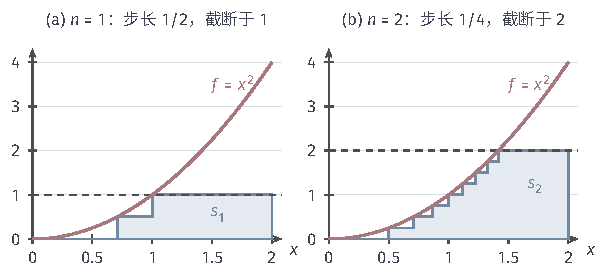
\includegraphics[width=102.634mm]{figures/02-abstract-mathematics/01-metric-and-measure/tikz/c3-dyadic-approximation/figure.pdf}
  \caption{二进分层逼近$f(x)=x^2$，$x\in[0,2]$。蓝色阶梯是$\varphi_n=2^{-n}\lfloor2^n\min\{f,n\}\rfloor$，虚线是截断高度$n$。(a)$n=1$，$\varphi_1$取值$0,0.5,1$；(b)$n=2$，$\varphi_2$取值$0,0.25,\dots,2$，断点为$\sqrt{k/4}$。阶梯始终位于曲线下方，且随$n$增大而升高。}
  \label{fig:meas-dyadic-approximation}
\end{figure}

这个逼近有三点要在下一章用到。第一，它从下方逼近，所以“下方简单函数的累计”自然成为非负函数积分的候选定义。第二，它单调递增，下一章将证明递增逼近的积分收敛到极限的积分。第三，它对每个非负可测函数都存在，不要求连续，也不要求有界；无界或取$+\infty$的函数由截断高度$n$逐步纳入。
